\section{Resultados}
\label{sec:resultados}

Esta seção apresenta os números sem interpretá-los; a leitura vai para a Seção
\ref{sec:discussao}. Todos os valores vêm de \texttt{resultados/}, gerado por
\texttt{python -m analise} sobre 300 repositórios, 18.389 releases e 20.117 episódios de
falha.

\subsection{RQ 01 a 04: as quatro métricas}

A Tabela \ref{tab:sintese} reúne mediana, quartis e IQR de cada métrica e variante, e a
Figura \ref{fig:violino} mostra a forma das distribuições. As quatro são fortemente
assimétricas: o lead time (a) vai de 1,2 h a mais de 50.000 h, com IQR de 880 h.

\begin{table}[ht]
\centering
\caption{Síntese das RQ 01 a 04: mediana, quartis e IQR por métrica e variante.}
\label{tab:sintese}
\small
\begin{tabular}{llrrrrr}
\toprule
\textbf{Métrica} & \textbf{Variante} & \textbf{n} & \textbf{Mediana} & \textbf{Q1} &
\textbf{Q3} & \textbf{IQR} \\
\midrule
Deployment frequency (rel./sem.) & única & 300 & 0,46 & 0,23 & 1,00 & 0,77 \\
\midrule
\multirow{2}{*}{Lead time (horas)} & (a) release & 300 & 324,91 & 116,73 & 996,90 & 880,17 \\
 & (b) commit & 300 & 411,81 & 128,16 & 1.844,33 & 1.716,16 \\
\midrule
\multirow{2}{*}{Change failure rate} & (a) CI & 300 & 0,056 & 0,013 & 0,133 & 0,120 \\
 & (b) entrega & 300 & 0,269 & 0,105 & 0,500 & 0,395 \\
\midrule
\multirow{2}{*}{Recuperação (horas)} & recuperados & 264 & 4,94 & 1,75 & 18,75 & 17,00 \\
 & limite inferior & 268 & 5,22 & 1,82 & 22,22 & 20,40 \\
\bottomrule
\end{tabular}
\end{table}

\begin{figure}[ht]
\centering
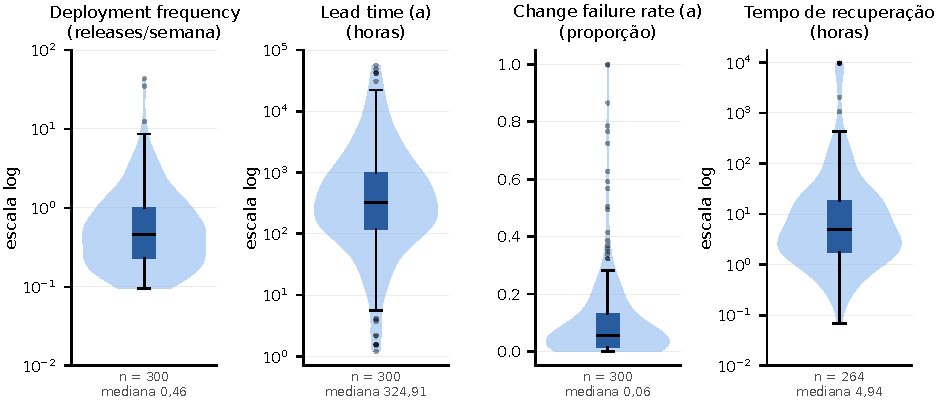
\includegraphics[width=\textwidth]{artigo_violino_metricas.pdf}
\caption{Distribuição das quatro métricas da C1. Violino para a forma, boxplot interno
para mediana e IQR. Unidades diferentes não dividem eixo: cada métrica tem seu painel, e
três delas estão em escala logarítmica.}
\label{fig:violino}
\end{figure}

\textbf{Censura e casos excluídos.} No lead time, 3.052 das 18.389 releases (16,6\%)
ficaram fora por motivo explícito: 3.026 por não trazerem commits novos em relação à
release anterior, 23 por não terem release anterior, 2 por \texttt{compare} com 404 e 1
por erro de \texttt{compare}. Nenhuma foi estimada ou tratada como intervalo zero. No
CFR (b), 246 releases publicadas nos últimos sete dias da janela ficaram fora do
denominador, em vez de contarem como sucesso, restando 18.143 avaliadas, das quais 10.974
falharam. No CFR (a) entraram 730.432 \emph{workflow runs} e ficaram de fora 60.959,
cancelados, em andamento ou com conclusão desconhecida. Na recuperação, dos 20.117
episódios de falha, 19.921 foram recuperados, 196 ficaram censurados e 124 com datas
contraditórias; 36 dos 300 repositórios não têm nenhum episódio recuperado e consistente,
e por isso ficam sem mediana. A proporção censurada por repositório tem mediana 0,00 e Q3
0,029. Tratando cada censurado como recuperado no fim da observação --- um limite
inferior do viés --- a mediana sobe de 4,94 h para 5,22 h, uma diferença de 0,28 h.

\subsection{Classificação DORA de referência (C1)}

A Tabela \ref{tab:c1} traz a distribuição das categorias. O CFR (a) concentra 234 dos 300
repositórios em \emph{Elite}; a classificação geral concentra-se em \emph{Medium} (154) e
\emph{High} (110), com apenas 9 \emph{Elite} e 27 \emph{Low}.

\begin{table}[ht]
\centering
\caption{Distribuição das categorias DORA na combinação C1 (300 repositórios).}
\label{tab:c1}
\small
\begin{tabular}{lrrrrr}
\toprule
\textbf{Métrica} & \textbf{Elite} & \textbf{High} & \textbf{Medium} & \textbf{Low} &
\textbf{Sem class.} \\
\midrule
Deployment frequency & 6 & 69 & 152 & 73 & 0 \\
Lead time (a) & 25 & 81 & 93 & 101 & 0 \\
Change failure rate (a) & 234 & 47 & 8 & 11 & 0 \\
Tempo de recuperação & 33 & 181 & 33 & 21 & 32 \\
\midrule
\textbf{Classificação geral} & \textbf{9} & \textbf{110} & \textbf{154} & \textbf{27} & \textbf{0} \\
\bottomrule
\end{tabular}
\end{table}

\subsection{RQ 05: frequência de entrega e taxa de falha}

Com o CFR (a), a correlação é desprezível e não significativa ($\rho = 0{,}071$,
$p = 0{,}222$, $n = 300$). Com o CFR (b), é moderada e fortemente significativa
($\rho = 0{,}615$, $p = 1{,}2 \times 10^{-32}$). A Figura \ref{fig:dispersao} mostra as
duas dispersões lado a lado.

\begin{figure}[ht]
\centering
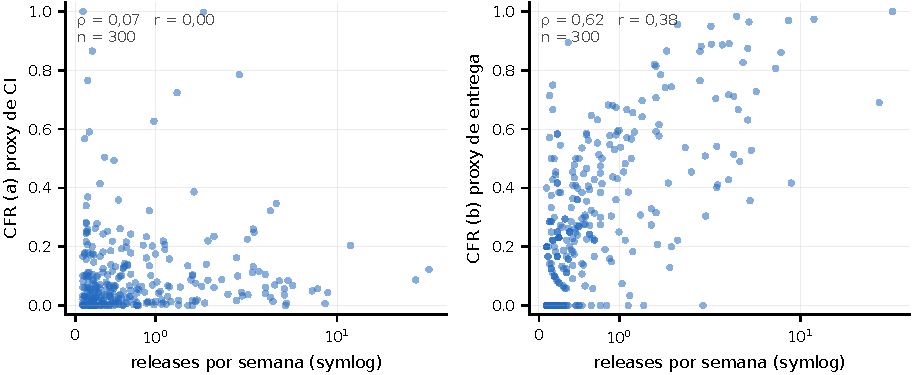
\includegraphics[width=\textwidth]{artigo_dispersao_df_cfr.pdf}
\caption{Frequência de entrega contra as duas variantes do CFR. À esquerda, o proxy de CI
não mostra relação; à direita, o proxy de entrega mostra associação positiva forte. Em
ambos os painéis, $\rho$ de Spearman e $r$ de Pearson.}
\label{fig:dispersao}
\end{figure}

O diagnóstico da janela de sete dias explica o segundo coeficiente: entre os
repositórios do quartil inferior de frequência, o intervalo mediano entre releases é de
27,9 dias e apenas 25,0\% dos intervalos cabem em sete dias; no quartil superior, o
intervalo mediano é de 1,39 dia e 87,7\% cabem na janela.

A Figura \ref{fig:correlacao} generaliza a análise para todos os pares de métricas, com
Spearman e Pearson lado a lado.

\begin{figure}[ht]
\centering
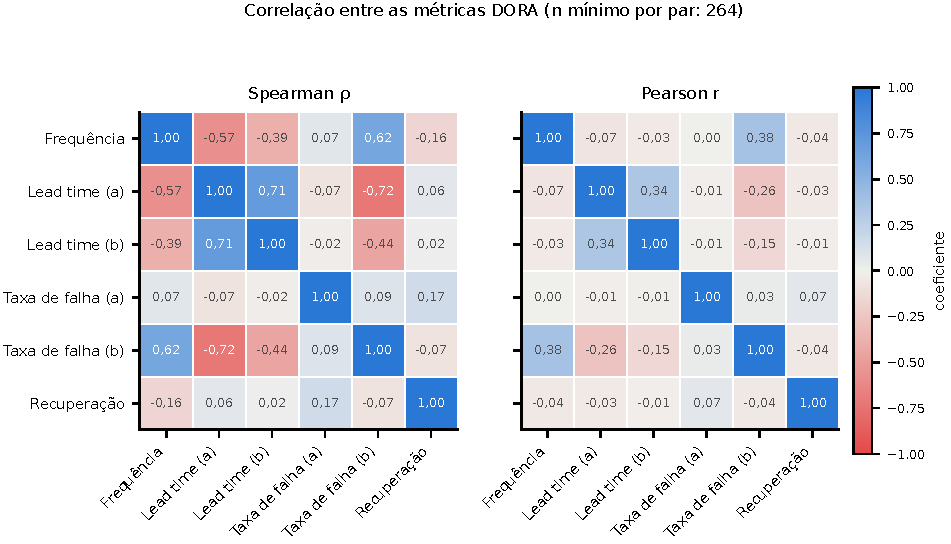
\includegraphics[width=\textwidth]{artigo_correlacao.pdf}
\caption{Correlação entre as métricas. O painel de Pearson é visivelmente mais pálido: em
DF $\times$ LT (a), $\rho = -0{,}57$ contra $r = -0{,}07$. As associações são monótonas,
não lineares.}
\label{fig:correlacao}
\end{figure}

\subsection{RQ 06: fatores associados ao desempenho}

Após a correção de Holm, quatro testes rejeitam a hipótese nula: linguagem contra
frequência de entrega ($\varepsilon^2 = 0{,}113$, efeito médio) e contra lead time (a)
($\varepsilon^2 = 0{,}164$, médio); número de contribuidores contra frequência
($\varepsilon^2 = 0{,}046$, pequeno) e contra lead time (a)
($\varepsilon^2 = 0{,}100$, médio). Estrelas não se associam a nenhuma das quatro
métricas após a correção. O fator idade não pôde ser testado: a estratificação não
produziu dois grupos válidos.

\subsection{RQ 07: sensibilidade às definições operacionais}

A Tabela \ref{tab:rq07} mostra o percentual de repositórios que mudam de categoria entre
cada par de combinações e o kappa ponderado correspondente.

\begin{table}[ht]
\centering
\caption{RQ 07: mudança de categoria geral entre combinações ($n = 300$).}
\label{tab:rq07}
\small
\begin{tabular}{llrrl}
\toprule
\textbf{Par} & \textbf{O que muda} & \textbf{Mudaram} & \textbf{\%} &
\textbf{$\kappa$ ponderado} \\
\midrule
C1 $\times$ C2 & unidade e variantes & 94 & 31,3 & 0,506 (moderada) \\
C1 $\times$ C3 & unidade (tag) & 73 & 24,3 & 0,651 (substancial) \\
C1 $\times$ C4 & só as variantes & 85 & 28,3 & 0,546 (moderada) \\
C2 $\times$ C4 & só a unidade & 22 & 7,3 & 0,878 (quase perfeita) \\
\bottomrule
\end{tabular}
\end{table}

Por métrica, o Change Failure Rate é o que mais se move: entre C1 e C2 muda em 72,3\% dos
repositórios, com $\kappa = -0{,}015$ --- concordância nula. A mediana do CFR passa de
0,056 na C1 para 0,274 na C2, um aumento de 3,88 vezes.

\subsection{RQ 08: taxa de retrabalho}

A taxa de retrabalho tem mediana 0,70 (IQR 0,41, $n = 300$): 12.020 das 18.366 releases
avaliadas foram classificadas como corretivas pela heurística v1. Sua correlação com o
CFR (b) é fraca ($\rho = 0{,}359$, $p = 1{,}5 \times 10^{-10}$). Avaliada contra a
amostra-ouro, a heurística v1 tem precisão 0,696, \emph{recall} 0,824 e F1 0,754.

\subsection{Fragilidade da classificação}

Em 259 dos 300 repositórios (86,3\%), mover uma única métrica um degrau muda a
classificação geral; em 53 a métrica mais próxima está a 5\% ou menos de um limite de
faixa, e em 31 as duas condições valem ao mesmo tempo. O caso mais extremo é
\texttt{ultralytics/ultralytics}, a 0,06\% do limite de 24 h do lead time.
